\documentclass{article}
\usepackage[T1]{fontenc}
\usepackage[utf8]{inputenc}
\usepackage[a4paper, total={6in, 8in}]{geometry}
%\usepackage[icelandic]{babel}
\usepackage{graphicx} %package to manage images

\usepackage{hyperref}
\usepackage{siunitx}
\usepackage{tabularx}
\usepackage{float}
\usepackage{xcolor}
\usepackage{listings}

\colorlet{mygray}{black!30}
\colorlet{mygreen}{green!60!blue}
\colorlet{mymauve}{red!60!blue}

\lstset{
  backgroundcolor=\color{gray!10},  
  basicstyle=\ttfamily,
  columns=fullflexible,
  breakatwhitespace=false,      
  breaklines=true,                
  captionpos=b,                    
  commentstyle=\color{mygreen}, 
  extendedchars=true,              
  frame=single,                   
  keepspaces=true,             
  keywordstyle=\color{blue},      
  language=c++,                 
  numbers=none,                
  numbersep=5pt,                   
  numberstyle=\tiny\color{blue}, 
  rulecolor=\color{mygray},        
  showspaces=false,               
  showtabs=false,                 
  stepnumber=5,                  
  stringstyle=\color{mymauve},    
  tabsize=3,                                     
  title=\lstname 
}

\title{Embedded Group Project\\ \large Project 4 - Kernel Space Encoder}

\author{Steinarr Hrafn Höskuldsson\\
Arnþór Gíslason\\
Andrew Madden\\
\\
Reykjavik University}
\date{October 2022}


\newcommand{\mycomment}[1]{}
\newcommand{\timerinterval}{5ms }

\begin{document}
\maketitle
 % how to comment, input image and code
\mycomment{
\begin{figure}[h]
    \centering
    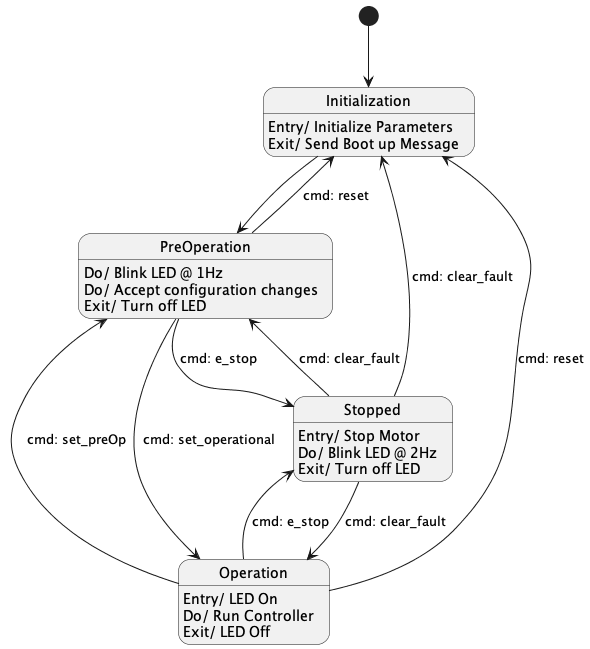
\includegraphics[width=0.75\textwidth]{Project3ControllerStateMachine/out/Project3ControllerStateMachine/docs/uml/uml.png}
    \caption{UML}
    \label{fig:UML}
\end{figure}

\lstinputlisting[caption=Defining 'ColorMatch' state, label={lst:colormatch}, language=Python, firstline=44, lastline=52]{LAB3/Basic.py}

}

\section{Part 1}
The header pins were soldered onto the Raspberry Pi Zero W2 and a voltmeter used to check that the pin orientation was correct.
\section{Part 2}
The four different methods for interfacing with the GPIO pins were tested.
\subsection{Test Setup}
A RIGOL DG1022 function generator was hooked up to the input pin and set to output a square wave with amplitude 3 volts and frequency 1kHz. A Rhode\&Schwartz RBT2004 oscilloscope was used to probe the input and output pins on different channels. The oscilloscope was then set to measure the time difference between rising edges.

With each method a screenshot of the oscilloscope was taken and the CPU load was read by running top in another terminal window.

\newpage
\subsection{Results}

\begin{table}[H]
\begin{tabular}{llll}
              & Mean delay & StdDev & CPU usage      \\
Shell script  & 3000 \mu s      & 1680 \mu s  & 19\%           \\
Read loop     & 8.5 \mu s    & 2.2 \mu s & 100\%          \\
Polling       & 147 \mu s     & 24   \mu s  & 0.3\%          \\
Kernel Module & 3.9 \mu s       & 0.48 \mu s  & Not detectable
\end{tabular}
\caption{}
\label{tab:my-table}
\end{table}
\begin{figure}[H]
    \centering
    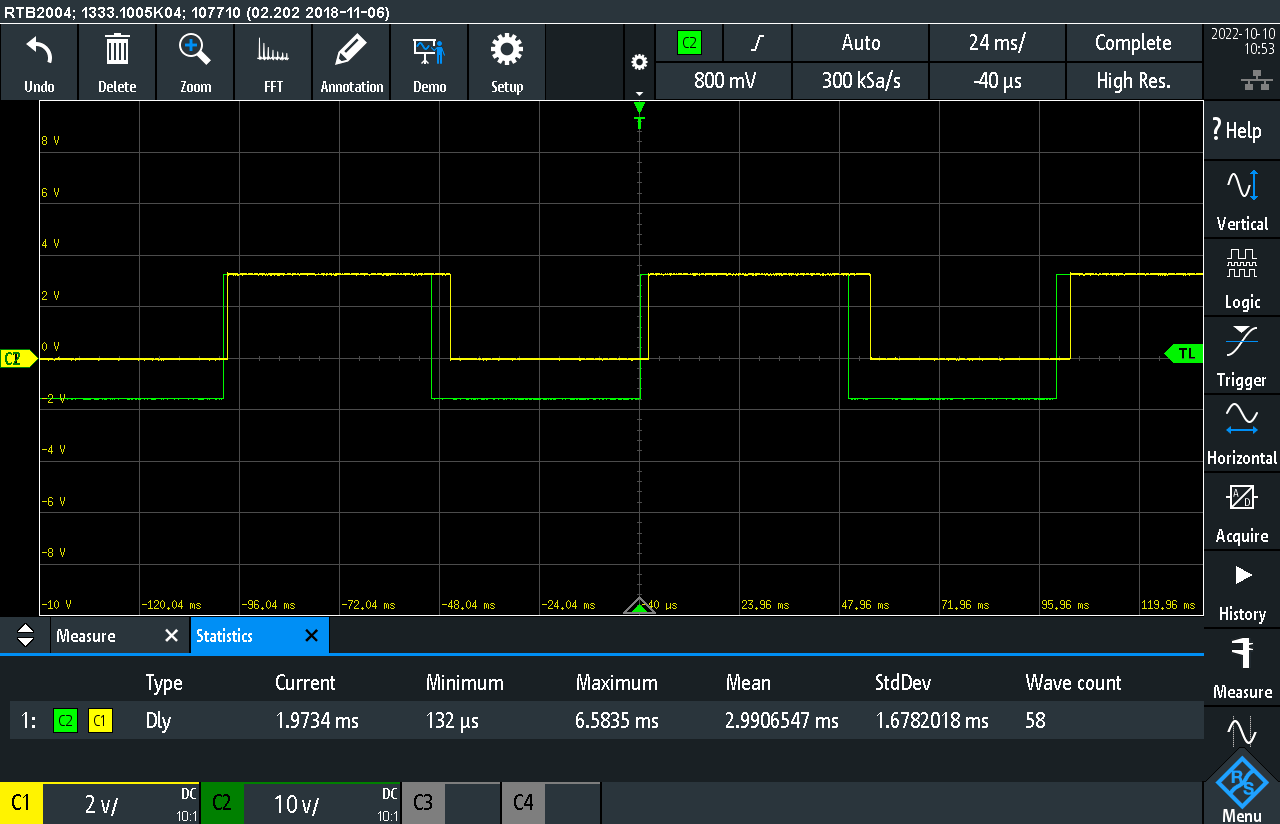
\includegraphics[width=0.75\textwidth]{Project4KernelSpaceEncoderDriver/part2_shell_mirror.PNG}
    \caption{Response time of a shell script utilizing sysfs to mirror a pin. CPU usage:19\%}
    \label{fig:shell}
\end{figure}

\begin{figure}[H]
    \centering
    \includegraphics[width=0.75\textwidth]{Project4KernelSpaceEncoderDriver/part2_2_read.PNG}
    \caption{Response of a c program reading from sysfs as fast as possible. CPU usage: 100\%}
    \label{fig:read}
\end{figure}

\begin{figure}[H]
    \centering
    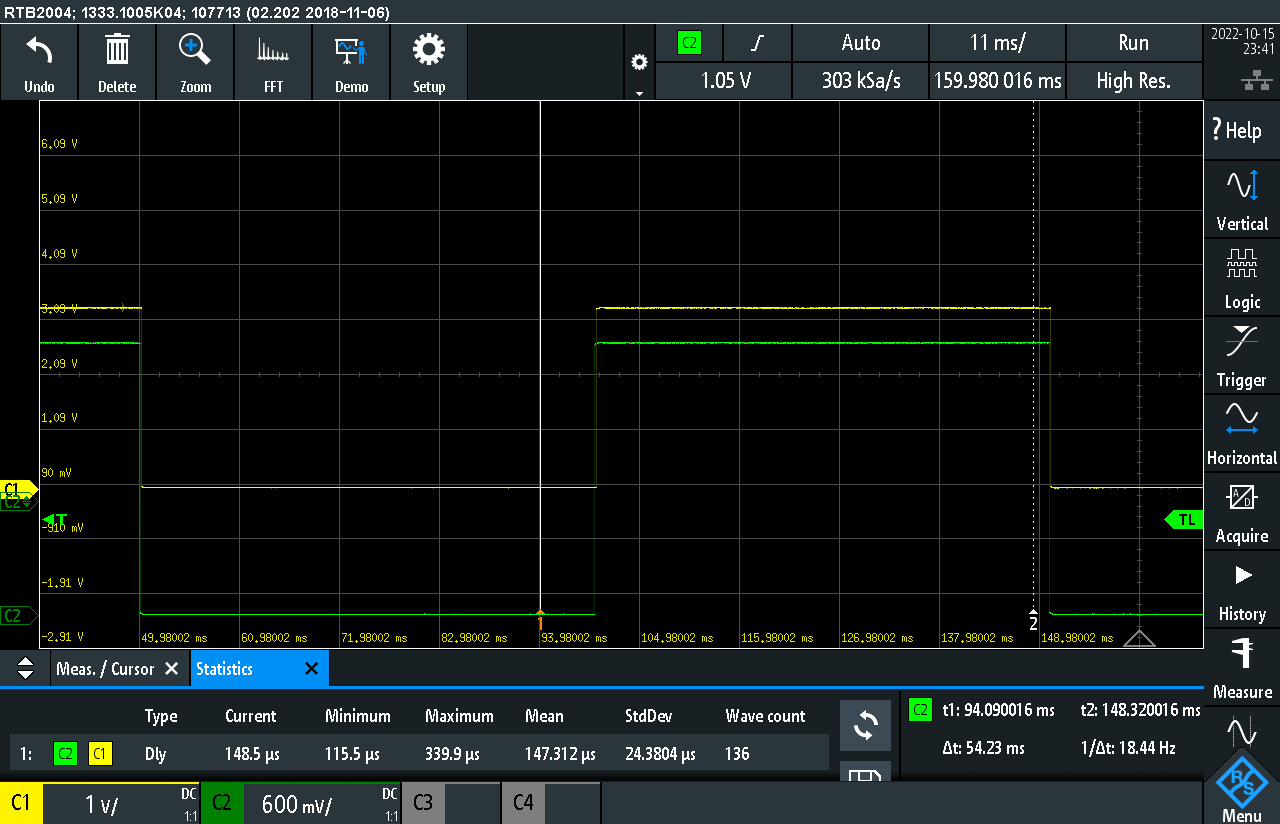
\includegraphics[width=0.75\textwidth]{Project4KernelSpaceEncoderDriver/Part2_3_poll.PNG}
    \caption{Response time of c program that uses polling and sysfs to detect changes to input pin. CPU usage: 0.3\%}
    \label{fig:poll}
\end{figure}

\begin{figure}[H]
    \centering
    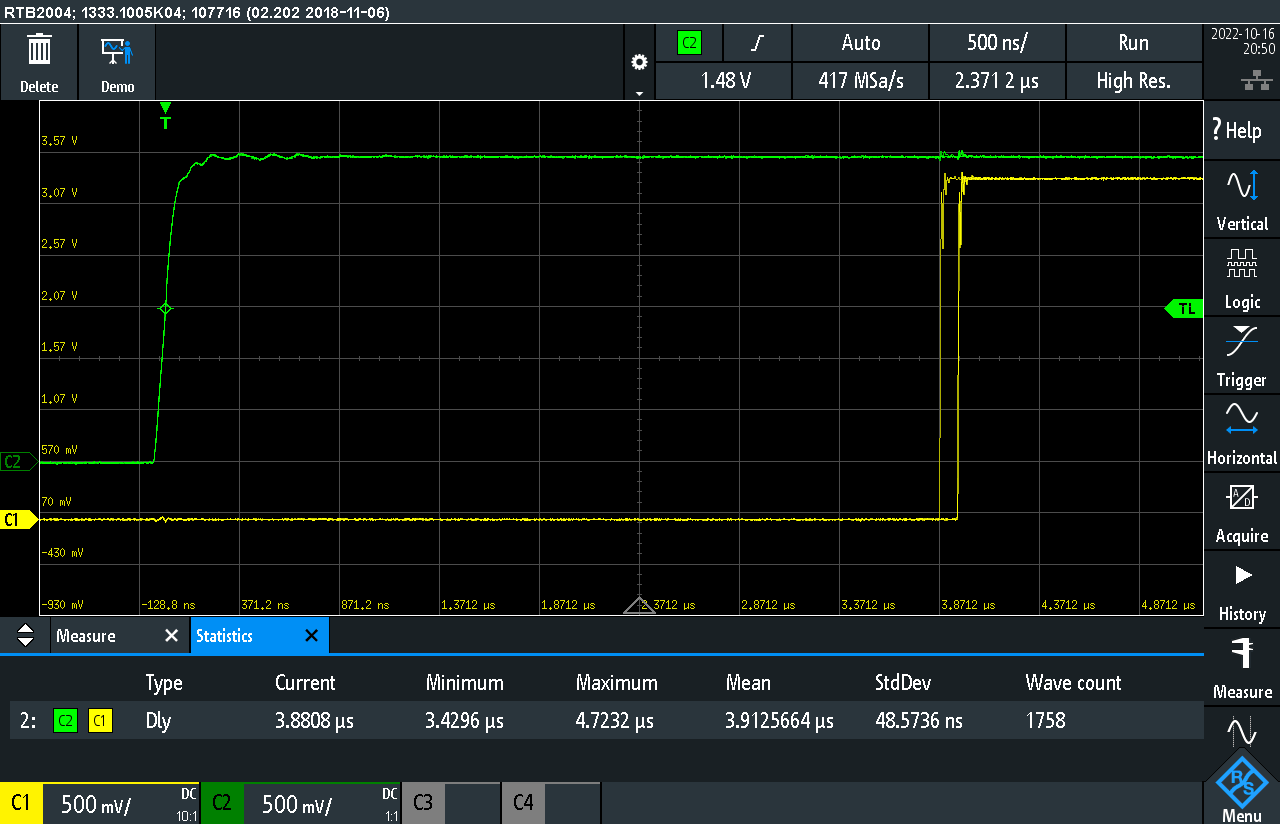
\includegraphics[width=0.75\textwidth]{Project4KernelSpaceEncoderDriver/part2_4_kernel.PNG}
    \caption{Response time of Linux Kernel Module that uses interrupts to detect changes to input pin. CPU usage: undetectable}
    \label{fig:kernel}
\end{figure}





\subsection{Discussion}
To count encoder pulses the Read Loop and Kernel Module methods would suffice however the read loop uses up an entire core of the CPU while the Kernel Module has no detectable affect on CPU usage. It might be interesting to implement the same behaviour in a c program using libgpiod.

\section{Part 3}

Implement the encoder counter in a kernel module, using interrupts.  Add a user-space application that reads the current counter value.

To test, attach the motor driver PWM input to the PWM output on pin 18 (see L4.5), attach the motor driver direction control pins (AIN1 & AIN2) to two digital output pins, and port the control loop from the previous project into a C++ application that uses your encoder driver.  You are not required to port the state behaviour.   For documentation, you can read a reference speed from the command line on program start and print the actual speed at the control rate. 

Evaluate the implementation.  How stable is the control rate?  Do you need to compensate for irregularities by using measured time in the integrator computation?

 


We printed the realtime of about 1000 runs of update and graphed both a histogram and a scatterplot to look at the jitter. On figure \ref{fig:scatterplotDelta} it may be seen that the time it takes varies from about 5.2ms to about .

\begin{figure}[h!t]
    \centering
    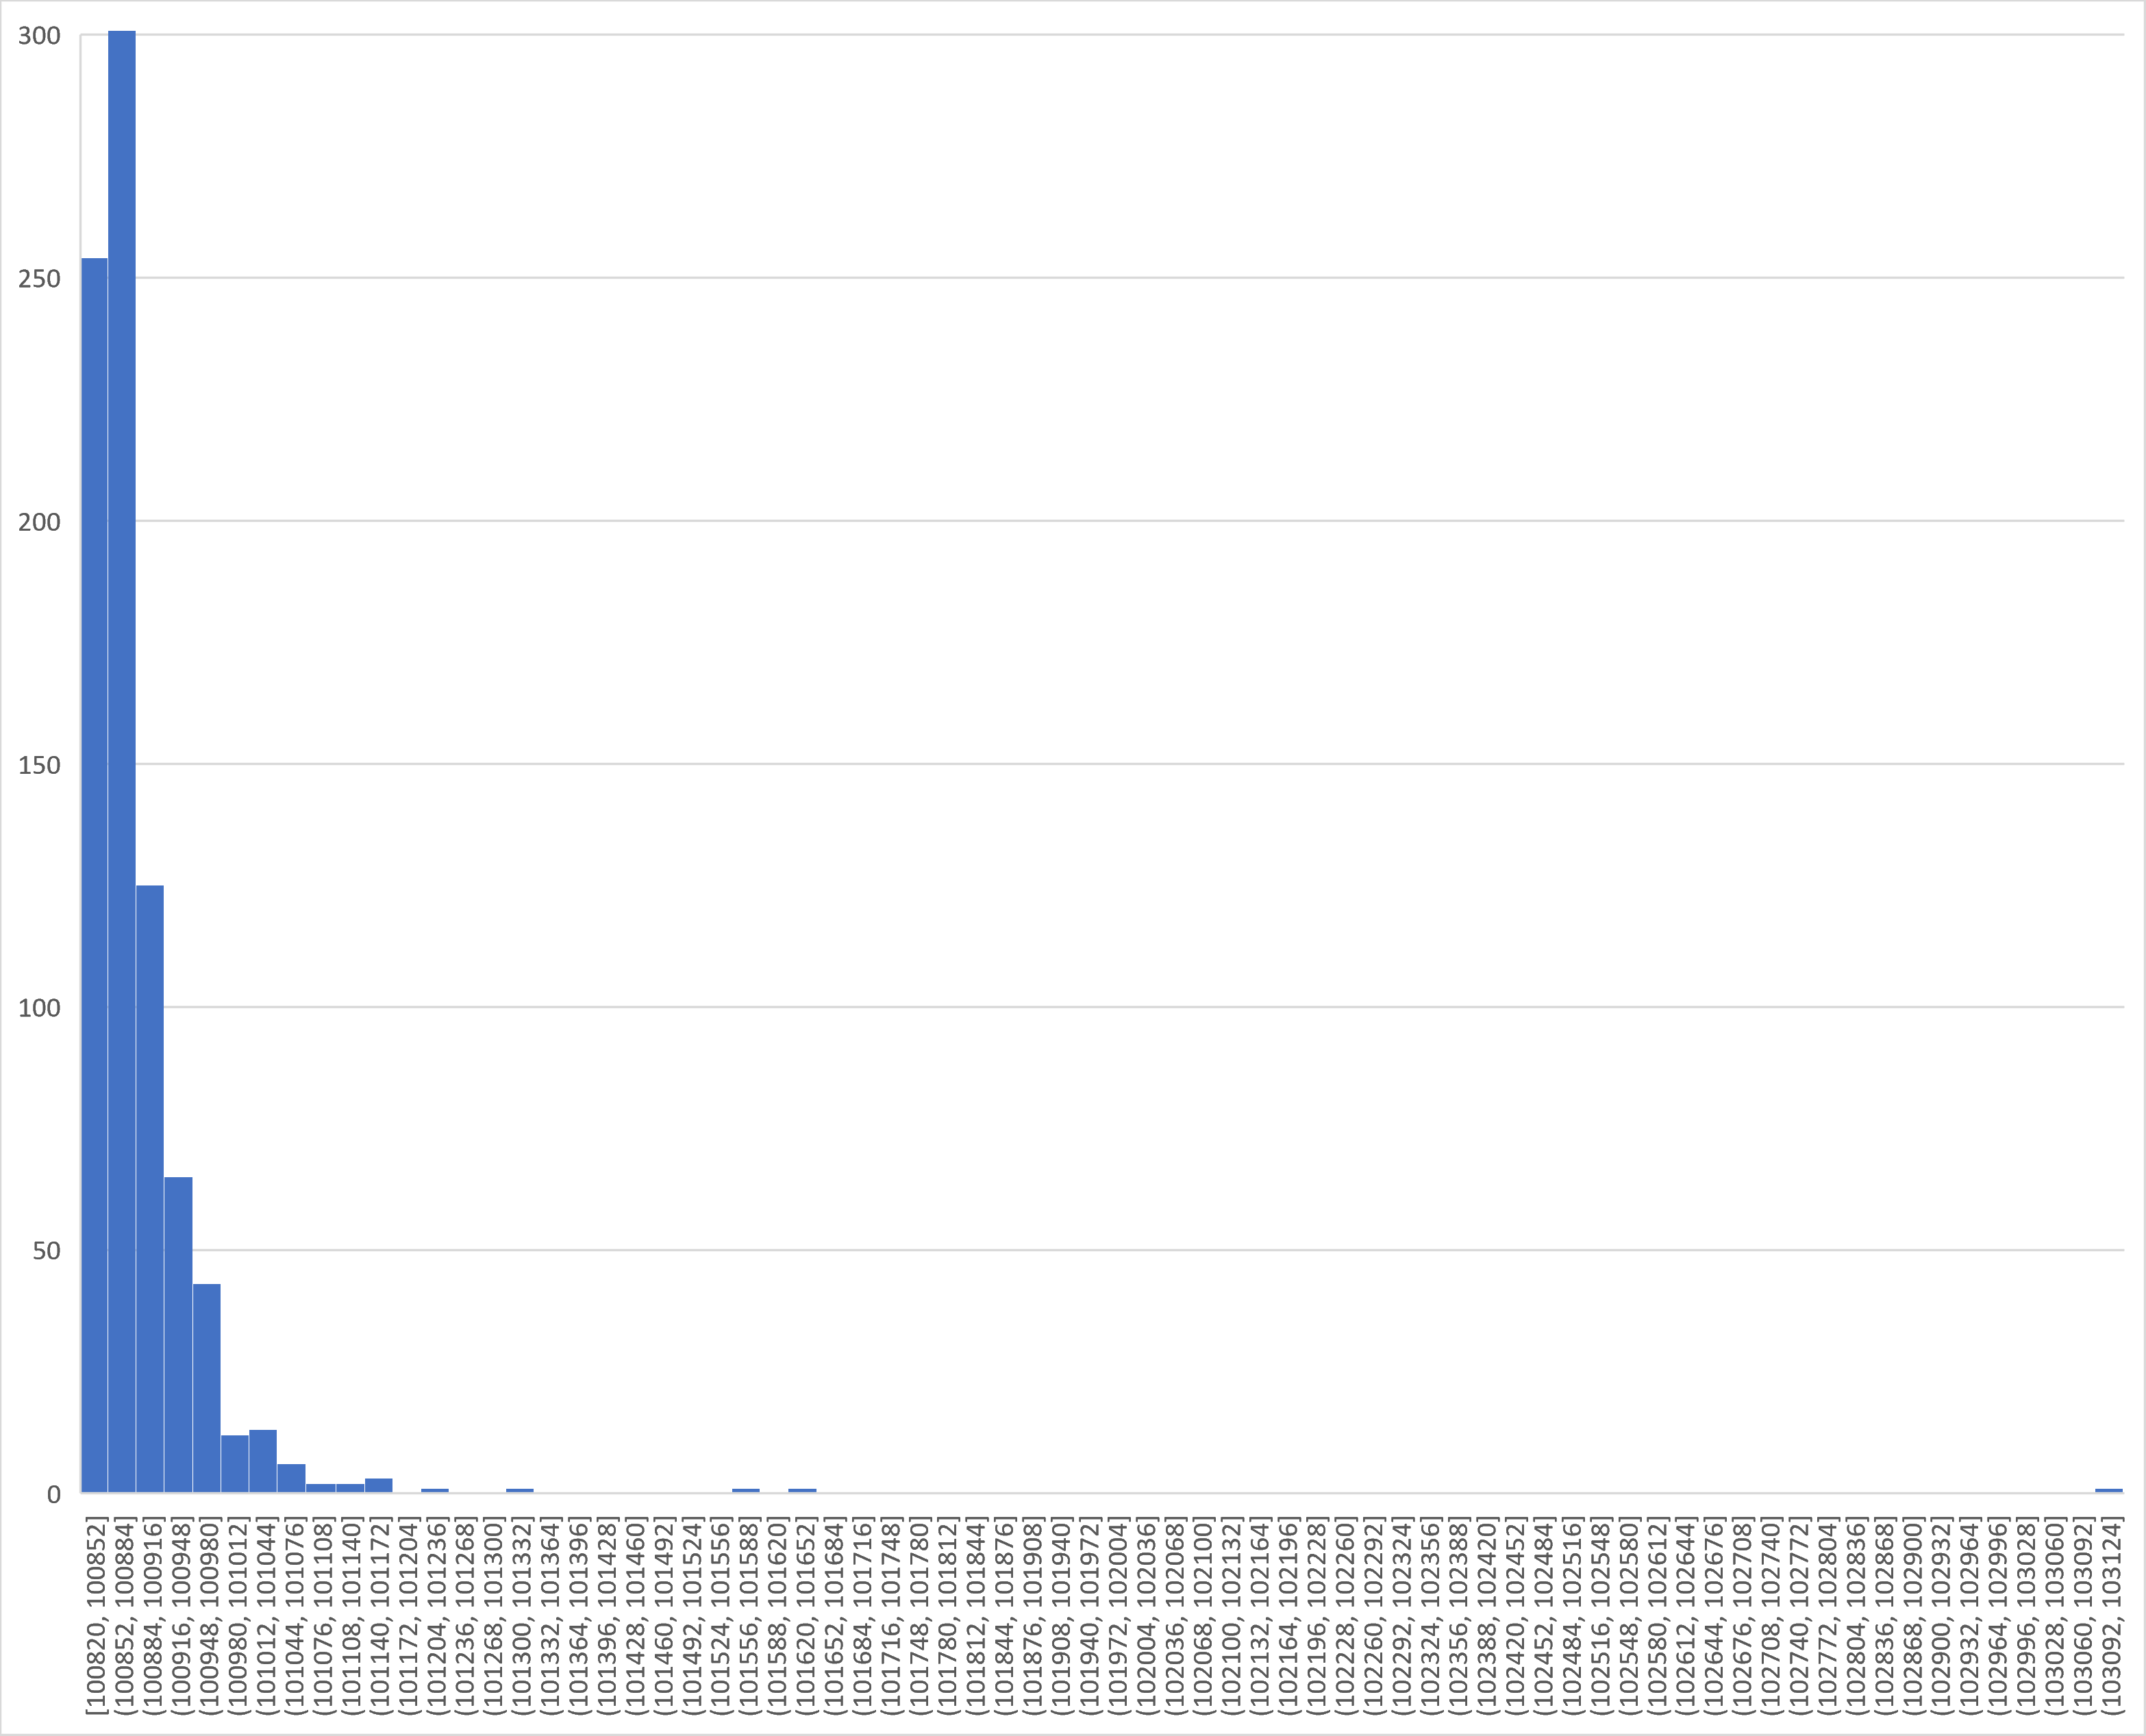
\includegraphics[width=0.75\textwidth]{Project4KernelSpaceEncoderDriver/histogram_timebetweenruns.png}
    \caption{histogram plot of delta time between runs of the PI controller}
    \label{fig:histogramDelta}
\end{figure}
\begin{figure}[h!]
    \centering
    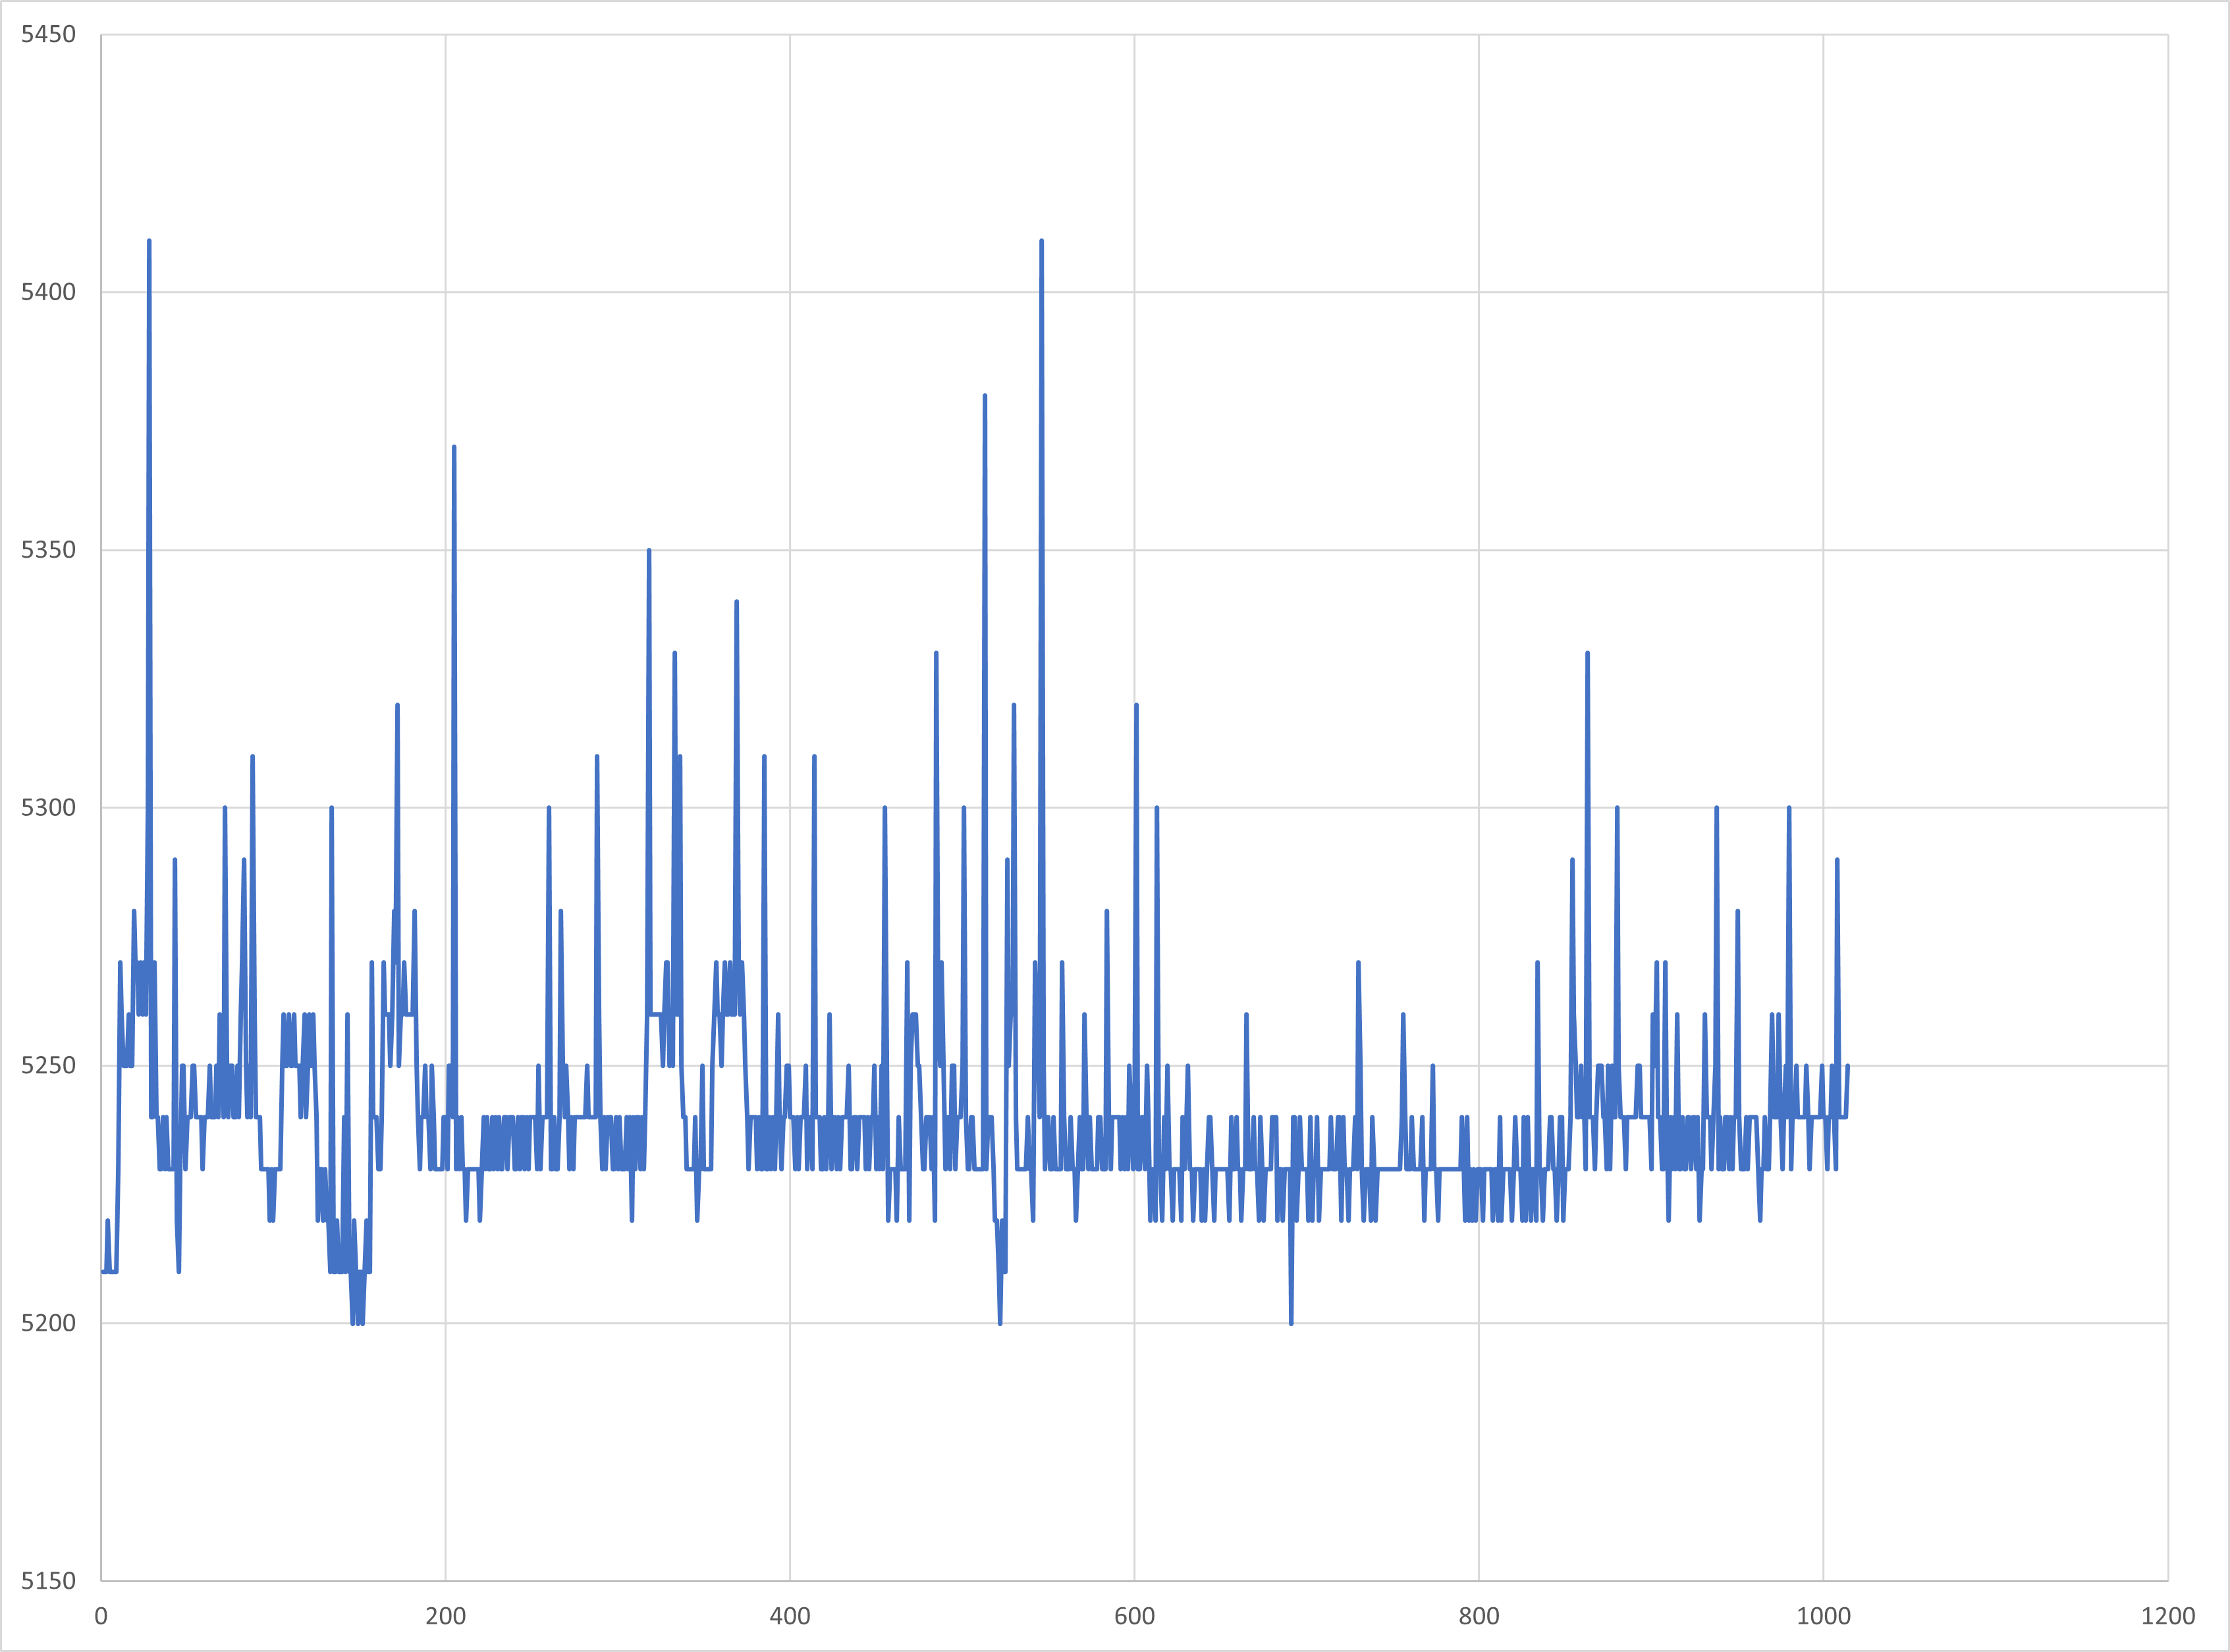
\includegraphics[width=0.75\textwidth]{Project4KernelSpaceEncoderDriver/scatterplot_between_runs.png}
    \caption{scatter plot of delta time between runs of the PI controller}
    \label{fig:scatterplotDelta}
\end{figure}
\url{https://youtu.be/eprVd00UXQw}
\newpage
\section*{Appendix}
\appendix

\newpage
\section{Code}\label{appendix:code}
A video of the control loop in action can be found at \url{}

The code used can be found on github at \url{}
\end{document}
